% Format teze zasnovan je na paketu memoir
% http://tug.ctan.org/macros/latex/contrib/memoir/memman.pdf ili
% http://texdoc.net/texmf-dist/doc/latex/memoir/memman.pdf
% 
% Prilikom zadavanja klase memoir, navedenim opcijama se podešava 
% veličina slova (12pt) i jednostrano štampanje (oneside).
% Ove parametre možete menjati samo ako pravite nezvanične verzije
% mastera za privatnu upotrebu (na primer, u b5 varijanti ima smisla 
% smanjiti 
\documentclass[12pt,oneside]{memoir}

% Paket koji definiše sve specifičnosti mastera Matematičkog fakulteta
\usepackage[latinica]{matfmaster}
%
% Podrazumevano pismo je ćirilica.
%   Ako koristite pdflatex, a ne xetex, sav latinički tekst na srpskom jeziku
%   treba biti okružen sa \lat{...} ili \begin{latinica}...\end{latinica}.
%
% Opicija [latinica]:
%   ako želite da pišete latiniciom, dodajte opciju "latinica" tj.
%   prethodni paket uključite pomoću: \usepackage[latinica]{matfmaster}.
%   Ako koristite pdflatex, a ne xetex, sav ćirilički tekst treba biti
%   okružen sa \cir{...} ili \begin{cirilica}...\end{cirilica}.
%
% Opcija [biblatex]:
%   ako želite da koristite reference na više jezika i umesto paketa
%   bibtex da koristite BibLaTeX/Biber, dodajte opciju "biblatex" tj.
%   prethodni paket uključite pomoću: \usepackage[biblatex]{matfmaster}
%
% Opcija [b5paper]:
%   ako želite da napravite verziju teze u manjem (b5) formatu, navedite
%   opciju "b5paper", tj. prethodni paket uključite pomoću: 
%   \usepackage[b5paper]{matfmaster}. Tada ima smisla razmisliti o promeni
%   veličine slova (izmenom opcije 12pt na 11pt u \documentclass{memoir}).
%
% Naravno, opcije je moguće kombinovati.
% Npr. \usepackage[b5paper,biblatex]{matfmaster}

% Pomoćni paket koji generiše nasumičan tekst u kojem se javljaju sva slova
% azbuke (nema potrebe koristiti ovo u pravim disertacijama)
\usepackage{pangrami}
\usepackage[x11names]{xcolor}
\usepackage{numprint}

% Paket koji obezbeđuje ispravni prikaz ćiriličkih italik slova kada
% se koristi pdflatex. Zakomentarisati ako na sistemu koji koristite ovaj
% paket nije dostupan ili ako ne radi ispravno.
\usepackage{cmsrb}

% Ostali paketi koji se koriste u dokumentu
\usepackage{listings} % listing programskog koda

% Datoteka sa literaturom u BibTex tj. BibLaTeX/Biber formatu
\bib{matfmaster-primer}

% Ime kandidata na srpskom jeziku (u odabranom pismu)
\autor{Luka B. Đorović}
% Naslov teze na srpskom jeziku (u odabranom pismu)
\naslov{Analiza slučajeva upotrebe relacionih i kolonski orijentisanih nerelacionih baza podataka}
% Godina u kojoj je teza predana komisiji
\godina{2024}
% Ime i afilijacija mentora (u odabranom pismu)
\mentor{др Saša \textsc{Malkov}, vanredni profesor\\ Универзитет у Београду, Математички факултет}
% Ime i afilijacija prvog člana komisije (u odabranom pismu)
\komisijaA{dr Nenad \textsc{Mitić}, redovni profesor\\ Универзитет у Београду, Математички факултет}
% Ime i afilijacija drugog člana komisije (u odabranom pismu)
\komisijaB{dr Ivana \textsc{Tanasijević}, доцент\\ Универзитет у Београду, Математички факултет}
% Ime i afilijacija trećeg člana komisije (opciono)
% \komisijaC{}
% Ime i afilijacija četvrtog člana komisije (opciono)
% \komisijaD{}
% Datum odbrane (obrisati ili iskomentarisati narednu liniju ako datum odbrane nije poznat)
\datumodbrane{15. јануар 2016.}

% Apstrakt na srpskom jeziku (u odabranom pismu)
\apstr{}

% Ključne reči na srpskom jeziku (u odabranom pismu)
\kljucnereci{анализа, геометрија, алгебра, логика, рачунарство, астрономија}

\begin{document}
% ==============================================================================
% Uvodni deo teze
\frontmatter
% ==============================================================================
% Naslovna strana
\naslovna
% Strana sa podacima o mentoru i članovima komisije
\komisija
% Strana sa posvetom (u odabranom pismu)
\posveta{Ovaj rad posvećujem...}
% Strana sa podacima o disertaciji na srpskom jeziku
\apstrakt
% Sadržaj teze
\tableofcontents*

% ==============================================================================
% Glavni deo teze
\mainmatter
% ==============================================================================

% ------------------------------------------------------------------------------
\chapter{Uvod}
% ------------------------------------------------------------------------------

Podaci su najstabilniji deo svakog sistema. Oni su reprezentacija činjenica i instrukcija u formalizovanom stanju spremnom za dalju interakciju, interpretaciju ili obradu od strane korisnika ili mašine. Iako kroz svoju istoriju računarstvo važi za oblast koja uvodi nove tehnologije i alate neverovatnom brzinom, to nije slučaj za svaku njenu granu. Postoje oblasti koje se kroz istoriju nisu menjale, ili su se slabo menjale i proširivale. Primera za to ima puno i oni su uglavnom usko vezani za funkcionalne principe koji se prožimaju kroz računarske mreže, kompilatore, operativne sisteme, sisteme za upravljanje podacima itd. 

Kada je reč o istoriji sistema za upravljanje podacima, mogu se izdvojiti tri faze: period pre relacionih sistema, vreme neprikosnovene vladavine relacionih sistema i nastanak alternativa relacionim sistemima pod grupnim nazivom \textit{NoSQL}.

Do nastanka relacionih sistema za upravljanje podacima, rukovanje podacima izvodilo se kroz pisanje i čitanje iz datoteka operativnog sistema. Rukovanje većim količinama podataka nije bilo standardizovano ni na koji način, već su se konvencije uvodile na nivou organizacija. Apolo sletanje na Mesec realizovano je koristeći ovakav vid rada sa podacima, što ovaj poduhvat čini utoliko neverovatnim \cite{ColumnarOriented}. 

S obzirom da je ovaj vid rada sa podacima imao mnogobrojne mane, među kojima je jedna od glavnih bila komplikovan pristup podacima, javile su se potrebe za unapređenjem. Najuspešniji je bio Edgar F. Codd \footnote{Edgar Frank "Ted" Codd (19 Avugst 1923 – 18 April 2003) Američki računarski naučnik }  koji je 1970. godine objavio rad pod imenom "\textit{A Relational Model of Data for Large Shared Data Banks}" kao rezultat sopstvenih istraživanja i teorija o organizaciji podataka.  Kao dokaz da je njegov model moguće implementirati pokrenut je System R \footnote{System R - sistem za rad sa podacima napravljen kao deo istraživačkog projekta IBM-a}, čiji je rezultat bio i pojava SQL-a (\textit{Structured Query Language}) kao standardizovanog jezika za rad sa podacima. Nakon toga pojavili su se Oracle i IBM sa svojim komercijalnim proizvodima za upravljanje relacionih baza podataka. Naredni period obeležio je rad sa podacima koristeći relacioni model.  

Ubrzanu digitalizacija, povećana dostupnost interneta, donela je sa sobom potrebu za obradom veće količine podataka. Sve ovo je pokazalo pojedine slabosti dosadašnjih sistema zasnovanih na relacionim modelima, koji nisu mogli u svim segmentima da odgovore na zahteve modernog doba. Ovi problemi obično poznati pod imenom: problemi velikih podataka (engl \textit{BigData problems}), doveli su do pojave niza novih modela i principa za čuvanje podataka, kojima je dodeljen  grupni naziv: nerelacione baze podataka (engl. \textit{NoSQL}).
Sistematizovanje ogromne količine fizičkog prostora na disku na kojem se podaci mogu čuvati i kasnije koristiti, kao i fleksibilnost strukture podataka sa kojima se radi, glavni su problemi tog vremena na koje su se fokusirale tehnologije nastale u \textit{NoSQL} pokretu.
Decenije vladavine  relacionih sistema za čuvanje podataka ostavile su dubok trag u praksama rada sa podacima, i sa razlogom predstavljaju standard i dan danas, te je eventualno usvajanje tehnologija nastalih u ovoj fazi i danas česta dilema mnogih stručnjaka. 

Kao važna grupa nerelacionih baza podataka izdvajaju se kolonski-orijentisane baze podataka. One su uvele tada nekonvencionalne koncepte čuvanja podataka po kolonama. To podrazumeva sekvencialno skladištenje vrednosti jedne kolone na disku, sa referencom na red kojem pripadaju. To sa sobom vuče razne mogućnosti za optimizaciju ali i nove pristupe modelovanja i organizacije podataka. Ovakav način skladištenja ispitavan je još davnih sedamdesetih godina XX veka, međutim u ranim godinama XXI veka došlo je do obnove interesovanja u akademskim ali i industrijskim krugovima. 

Nijedan od navedenih koncepata nije univerzalno rešenje, zato je bitno postojanje sadržaja koji se bave analizom slučajeva upotrebe tih tehnologija. Pored teorijske analize koja se može pronaći u relevantnim javnim dokumentacijama korisno je imati i konkretne implementacije testova čiji se rezultati mogu iskoristiti kako bi se povukle paralele u skladu sa potrebama realnih  sistema. 

Cilj ovog rada je analiza i upoređivanje slučajeva upotrebe relacionih i kolonski orijentisanih baza podataka. Rad će se sastojati iz teorijskog opisa navedenih tehnologija kao i opisa konkretnih predstavnika baza podataka koji će biti korišćeni. Na osnovu teorijskih izbora i istraživanja biće analizirani različiti slučajevi upotrebe. 


% ------------------------------------------------------------------------------
\chapter{Modeli podataka}
\label{chp:razrada}
\section{Relacioni model}
\subsection{Opšte karakteristike}
Relacioni model je najpopularniji model za rad sa podacima. On podatke kao i veze izmedju njih predstavlja kroz skup relacija koje predstaljaju skupove torki. Da bi jedan skup torki ili vrsta bila validna relacija u relacionom modelu, ona mora ispunjavati sledeće uslove:

\begin{enumerate}
\item[\textbullet] Presek kolone i vrste jedinstveno određuje vrednosnu ćeliju.

\item[\textbullet] Sve vrednosne ćelije jedne kolone pripadaju nekom zajedničkom skupu. 

\item[\textbullet] Svaka kolona ima jedinstveno ime.

\item[\textbullet] Ne postoje dve identične vrste jedne tabele. 
\end{enumerate}

Iako ovakva formalizacija relacije jeste intuitivna (usled istorijskog uticaja koji je relacioni model ostavio na ideju organizacije podataka) ona je neophodna za  definisanje složenijih pojmova. 

\subsection{Koncept ključa relacionog modela}

Skup kolona relacije za koji važi da dva reda te relacije nemaju identične vrednosti za svaku kolonu iz tog skupa naziva  se \textit{natključ} relacije. Svaki minimalan natključ naziva se \textit{ključ kandidat}. Svaka relacija može imati više ključeva kandidata, a jedan on njih se bira za  \textit{primarni ključ} koji mora imati definisanu vrednost za svaku njegovu kolonu.
\textit{Strani ključ} je kolona ili skup kolona čije vrednosti predstavljaju referencu na određeni red neke druge relacije. On uzima vrednost primarnog ključa torke na koju pokazuje. 

Primarni i strani ključ igraju veliku ulogu u očuvanju integriteta baze podataka o čemu će biti reči u nastavku.

\subsection{Integritet relacionog modela}

Integritet relacionog modela predstavlja uslove koje podaci treba da zadovolje kako bi stanje u bazi ostalo konzistentno \cite{URBP} . On se drugačije naziva i "unutrašnja konzistentost" s obzirom da predstavlja aspekte koji mogu da se provere bez konsultovanja domena (npr. ne može se proveriti da li je ime studenta u tabeli ispravno bez konsultovanja domena, ali može se garantovati da će neophodni podaci biti prisutni, uzimati vrednosti iz predviđenog skupa vrednosti i sl.) . Provera integriteta se izvršava implicitno ili eksplicitno prilikom svakog ažuriranja baze podataka. Postoji više vrsta integriteta u relacionom modelu:  \textit{integritet entiteta}, \textit{integritet domena}, \textit{integritet neposojeće vrednosti} i \textit{referencijalni integritet}.

 \textit{Integritet entiteta} kaže da svaka torka mora imati definisan primarni ključ bez nedostajućih vrednosti.

\textit{Integritet domena} predstavlja uslov da za svaku kolonu postoji unapred poznati skup vrednosti koje ona može uzimati.

\textit{Integritet nepostojeće vrednosti} dodeljuje se kolonama koje  ne smeju uzimati nedostajuću vrednost.

\textit{Referencijalni integritet} nalaže da za svaki strani ključ relacije mora postojati torka u tabeli na koju pokazuje čiji se primarni ključ poklapa sa njim.

\subsection{PostgreSQL}


PostgreSQL je objektno-relacioni sistem za upravljanje bazama podataka koji je nastao, a kasnije i bio razvijan na Berkliju, Univerzitet Kalifornija. PostgreSQL je otvorenog koda sa velikom SQL podrškom kao i modernim funkcionalnostima poput: kompleksnih upita, okidača, izmenjivih pogleda, transakcionog integriteta i mnogih drugih. Postgres nudi širok spektar proširenja od strane korisnika poput dodavanja novih tipova podataka, funkcija, operatora, agregatnih funkcija itd. 

Kao takav, PostgreSQL je pogodan sistem za čuvanje najkompleksnijih podataka i veza između njih. Mogućnost kreiranja procedura na samoj bazi u integrisanoj SQL sintaksi, daje široke mogućnosti optimizacije aplikacija. 

PostgresSQL koristi server-klijent model funkcionisanja. Sastoji se iz serverskog i klijentskog dela procesa. Serverski deo rukuje fajlovima baze podataka, prihvata konekcije, izvršava konkretne operacije nad bazom. Klijentski deo predstavlja aplikaciju kojom korisnik može da komunicira i rukuje podacima na serverskom delu. Klijent i server komunkciraju preko TCP/IP protokola. Serverski deo može raditi sa više konekcija istovremeno tako što svaka klijentska konekcija radi kao zaseban proces.

Postgres iza sebe ima razvijenu društvenu zajednicu, pa samim tim ima dosta izvora i dokumentacije koje mogu olakšati učenje ovog sistema \cite{PostgreSQLUpAndRunning}. 

\section{Kolonski-orijentisani model}
% ------------------------------------------------------------------------------
\subsection{Opšte karakteristike}

Susret sa Big Data problemima doveo do potrebe za tabelama koje imaju ogroman broj kolona, i ogroman broj redova u okviru tih tabela. Novonastali zahtevi ukazali su na problem kod postojećih  relacionih modela. Svaki upit nad tabelom podrazumevao je dohvatanje svih kolona jednog reda, gde bi se filtriranje nepotrebnih kolona izvršavalo nakon što su se sve kolone učitale u memoriju. Ovo je bila samo jedna od motivacija za implemetanciju sistema zasnovanih na kolonski orijentisanom modelu koji je dizajniran tako da ovakav problem izbegne i uz to donese i druga poboljšanja o kojima će biti reči u nastavku.

Kolonski orijentisan model podatke na disku skladišti po kolonama, a ne po redovima kao što je to slučaj kod relacionh modela, slika 2.1. Sve vrednosti kolone svih redova skladište se jedna do druge, a na konkretnu vrednosnu ćeliju referiše se pomoću ključa konkretnog reda kao i kolone čiju vrednost želimo da pročitamo. Ovakav dizajn doveo je do toga da za dohvatanje određenog skupa kolona nema potrebe da čitamo sve vrednosti tog reda, već je dovoljno da znamo konkretan ključ tog reda kao i imena kolona čije vrednosti želimo da pročitamo i tako izbegnemo višak operacija čitanja sa diska.

Ovakav vid skladištenja podataka sa sobom nosi veliki potencijal za primenu raznih algoritama za kompresiju podataka.  Kompresija nad sličnim podacima koji se nalaze na uzastopnim adresama u memoriji, omogućava izbegavanje čuvanja složenih meta informacija u okviru struktura koje se koriste za tu kompresiju, što ovaj model čini posebno pogodnim za njihovu primenu.

Kolonski orijentisan model kao i većina ostalih nerelacionih modela, nudi fleksibilnost strukture podataka koja se ogleda u neograničenom broju kolona, što daje dosta prostora za eksperimentisanje sa dizajnom baze podataka. Primer toga biće prikazan u okviru analize OLAP slučaja upotrebe. 
\begin{figure}[!ht]
  \vspace*{4cm}
  \centering
  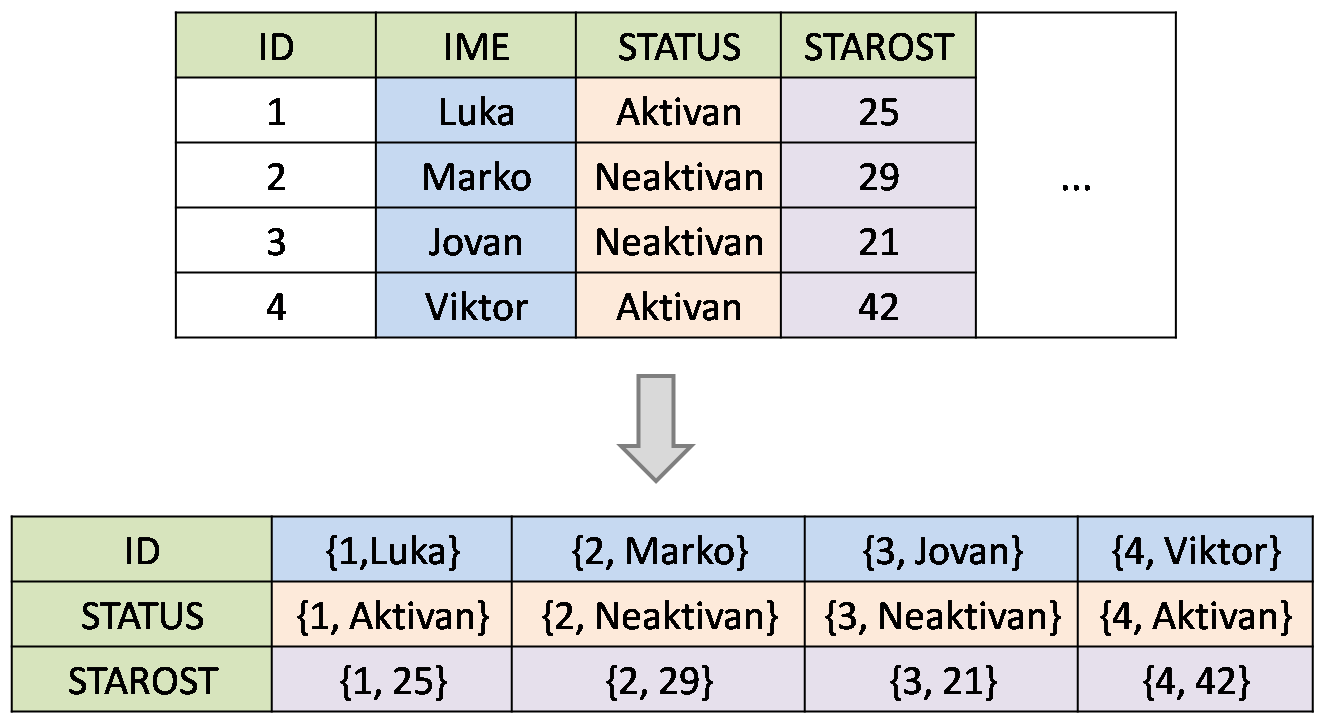
\includegraphics[width=0.9\textwidth]{relational-column-oriented.png}
  \caption{Kolonski orijentisan format}
  \label{fig:grafikon}
\end{figure}

\subsection{Popularni algoritmi kompresije kolonski orijentisanog modela}

Neke od najpoznatijih algoritama kompresije koje kolonski orijentisan model koristi i koji će biti opisani u nastavku jesu: enkodiranje zasnovano na rečniku, enkodiranje po broju ponavljanja i delta enkoding. Važno je napomenuti da relacioni modeli imaju svoje mehanizme kompresije podataka koji u ovom radu nisu analizirani.

Enkodiranje zasnovano na rečniku (engl. \textit{Dictionary based encoding}), slika 2.2., funkcioniše tako što se napravi mapa vrednosti koja sadrži svaku vrednost kolone koja je prisutna na disku. Kao vrednost kolone tada se ne upisuje konkretna vrednost, već ključ iz rečnika koji je mapiran na tu vrednost. Veličina ključa je srazmerna veličini mape, te je ovaj vid kompresije najpogodniji za kolone koje imaju mali broj vrednosti koje se ponavljaju.

\begin{figure}[!ht]
  \centering
  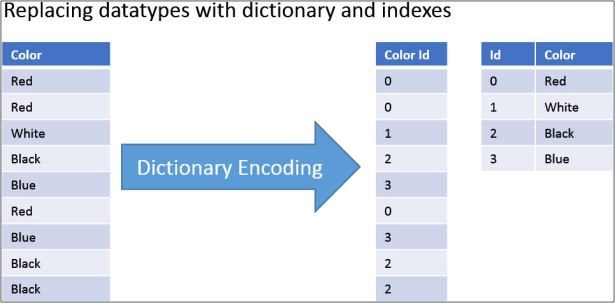
\includegraphics[width=0.9\textwidth]{DictionaryEncoding.jpg}
  \caption{Enkodiranje zasnovano na rečniku}
  \label{fig:grafikon}
\end{figure}


Enkodiranje po broju ponavljanja  (engl. \textit{Run Length Encoding}) , slika 2.3., funkcioniše tako što se uz svaku vrednost koja se ponavlja čuva i broj ponavljanja te vrednosti. Na taj način se izbegava pojava duplikata na uzastopnim adresama u memoriji. Ovaj vid kompresije najpogodniji je za kolone koje su sortirane.
\pagebreak



\begin{figure}[!ht]
  \centering
  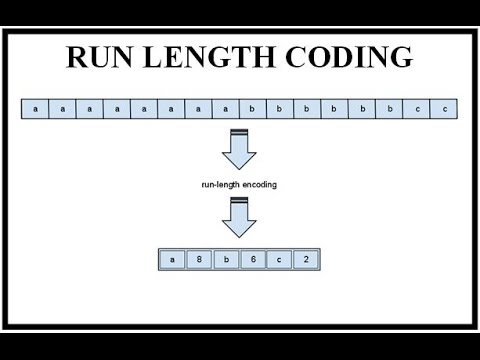
\includegraphics[width=0.9\textwidth]{run-length-encoding.jpg}
  \caption{Enkodiranje po broju ponavljanja}
  \label{fig:grafikon}
\end{figure}


Delta enkoding, algoritam kompresije, slika 2.4. funkcioniše tako što se u kolonama ne čuvaju same vrednosti već razlike između uzastopnih vrednosti. Očigledan primer primene ove kompresije je datumska kolona koja za vrednosti uzima uzastupne datume. U tom slučaju  je dovoljno da izaberemo neki referentni datum i da za ostale kolone čuvamo razliku u odnosu na taj datum.

\begin{figure}[!ht]
  \centering
  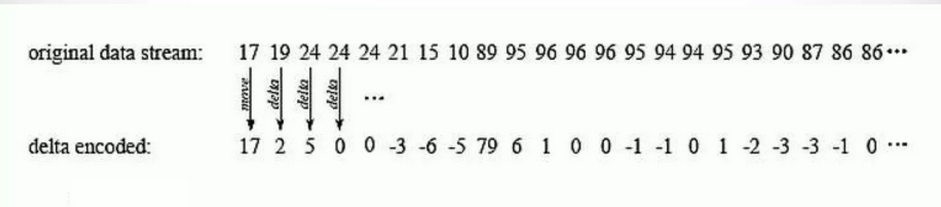
\includegraphics[width=0.9\textwidth]{delta-encoding.png}
  \caption{Delta enkoding}
  \label{fig:grafikon}
\end{figure}

\subsection{HBase}

HBase je distribuirana kolonski orijentisana nerelaciona baza podataka nastala 2007. godine kao prototip \textit{BigTable} baze koja je modelovana u okviru Google-ovog članka 2006 \cite{BigTable}. 

Model podataka koji HBase koristi podrazumeva da se svaka tabela sastoji iz familije kolona, a da svaka familija kolona sadrži određeni skup kolona.  S obzirom da će se kolone koje pripadaju jednoj familiji sladištiti blizu na disku, cilj je da atributi, odnosno kolone koje su po prirodi slične pripadaju istoj familiji kolona, kako bi se nad njima mogli primeniti algoritmi kompresije. Hbase nudi fleksibilnost strukture podataka, što znači da da bismo neki podatak skladištili ne moramo unapred da definišemo skup kolona koji pripada nekoj tabeli , ali moramo definisati skup familija kolona te tabele.

HBase ne podržava indekse, ali su ključevi svih redova sortirani rastuće, tako da se koristi binarna pretraga za pretragu vrednosti po ključu reda kojem pripada. Ovakvo ponašanje daje na važnosti dizajniranju ključa kako bi svako čitanje podataka išlo preko ključa ili njegovog prefiksa. 

Vrednosnu ćeliju u HBase tabeli određuje ključ reda, ime kolone te vrednosne ćelije, kao i familija kojoj kolona pripada, slika 2.5.

HBase nije ACID baza podataka, ali nudi sledeće garancije \cite{hbaseACID}: 

\begin{enumerate}
\item[\textbullet] Atomičnost pri radu sa jednim redom tabele koja se ogleda što će svaka  svaka izmena reda u potpunosti uspeti, ili u potpunosti propasti.
\item[\textbullet] Svako čitanje reda iz tabele vratiće stanje reda koje je bilo aktuelno najranije u trenutku kada je čitanje započeto. 
\end{enumerate}

\begin{figure}[!ht]
  \centering
  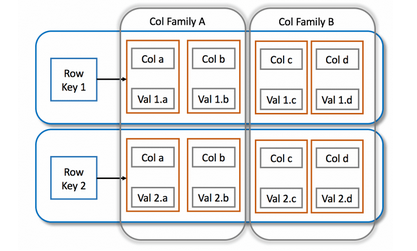
\includegraphics[width=0.7\textwidth]{colFamily.png}
  \caption{Hbase model}
  \label{fig:grafikon}
\end{figure}

Arhitektura HBase klastera sastoji se iz dve glavne komponente:  master server i region server. 

Master server  sadrži servise koji rade sa metainformacijama o tabelama i familijama kolona. Uloga Master servera jeste da zahtev za podacima za konkretan ključ reda može da delegira na odgovarajući region server. Master server u te svrhe koristi \textit{Zookeeper} \cite{BigTable} servis. Po potrebi master server takođe radi balansiranje opterećenja klastera. 

Region server implementira servise koji direktno rade sa podacima. On organizuje regione (jedan region čine redovi u nekom rasponu vrednosti ključeva), čita i upisuje u HFile fajlove (HFile je fajl koji je rezultat kolonski orijentisanog formata, a koji se skladišti na disku). Svaka izmena koja treba da se izvrši na disku prvo se upisuje u WAL (engl \textit{Write ahead log}), a nova izmenjena vrednost se upisuje u MemStore fajl. Kada se MemStore fajl upuni tek tada se izmene reflektuju u jedan HFile koji dalje ide na HDFS ili lokalni fajl sistem u zavisnosti od režima rada. 

HBase dozvoljava dva režima: samostalan i distribuirani režim.

U samostalnom režimu HFile fajlove može čuvati na lokalnom fajl sistemu i korišćenje HDFS-a je opciono, slika 2.6.

Sa druge strane distribuiranom režimu neophodno je korišćenje HDFS-a za skladištenje, slika 2.7. 

\begin{figure}[!ht]
  \centering
  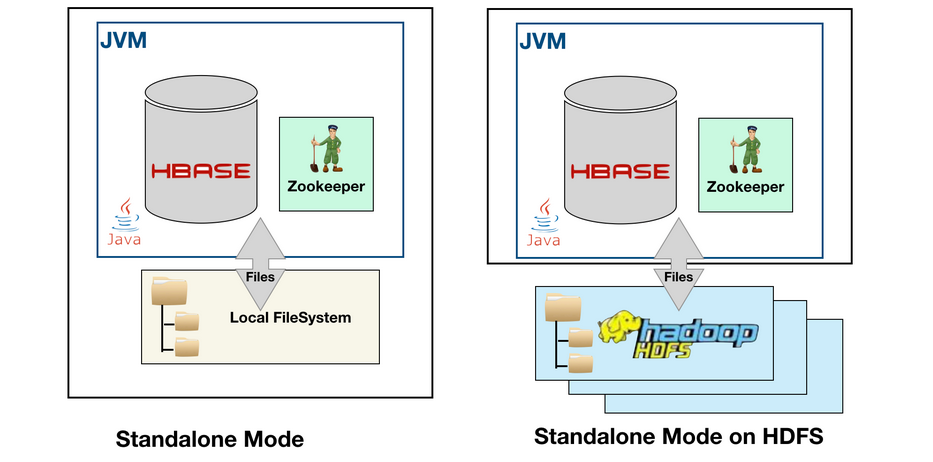
\includegraphics[width=0.9\textwidth]{hbase-standalone.png}
  \caption{HBase standalone}
  \label{fig:grafikon}
\end{figure}

\begin{figure}[!ht]
  \centering
  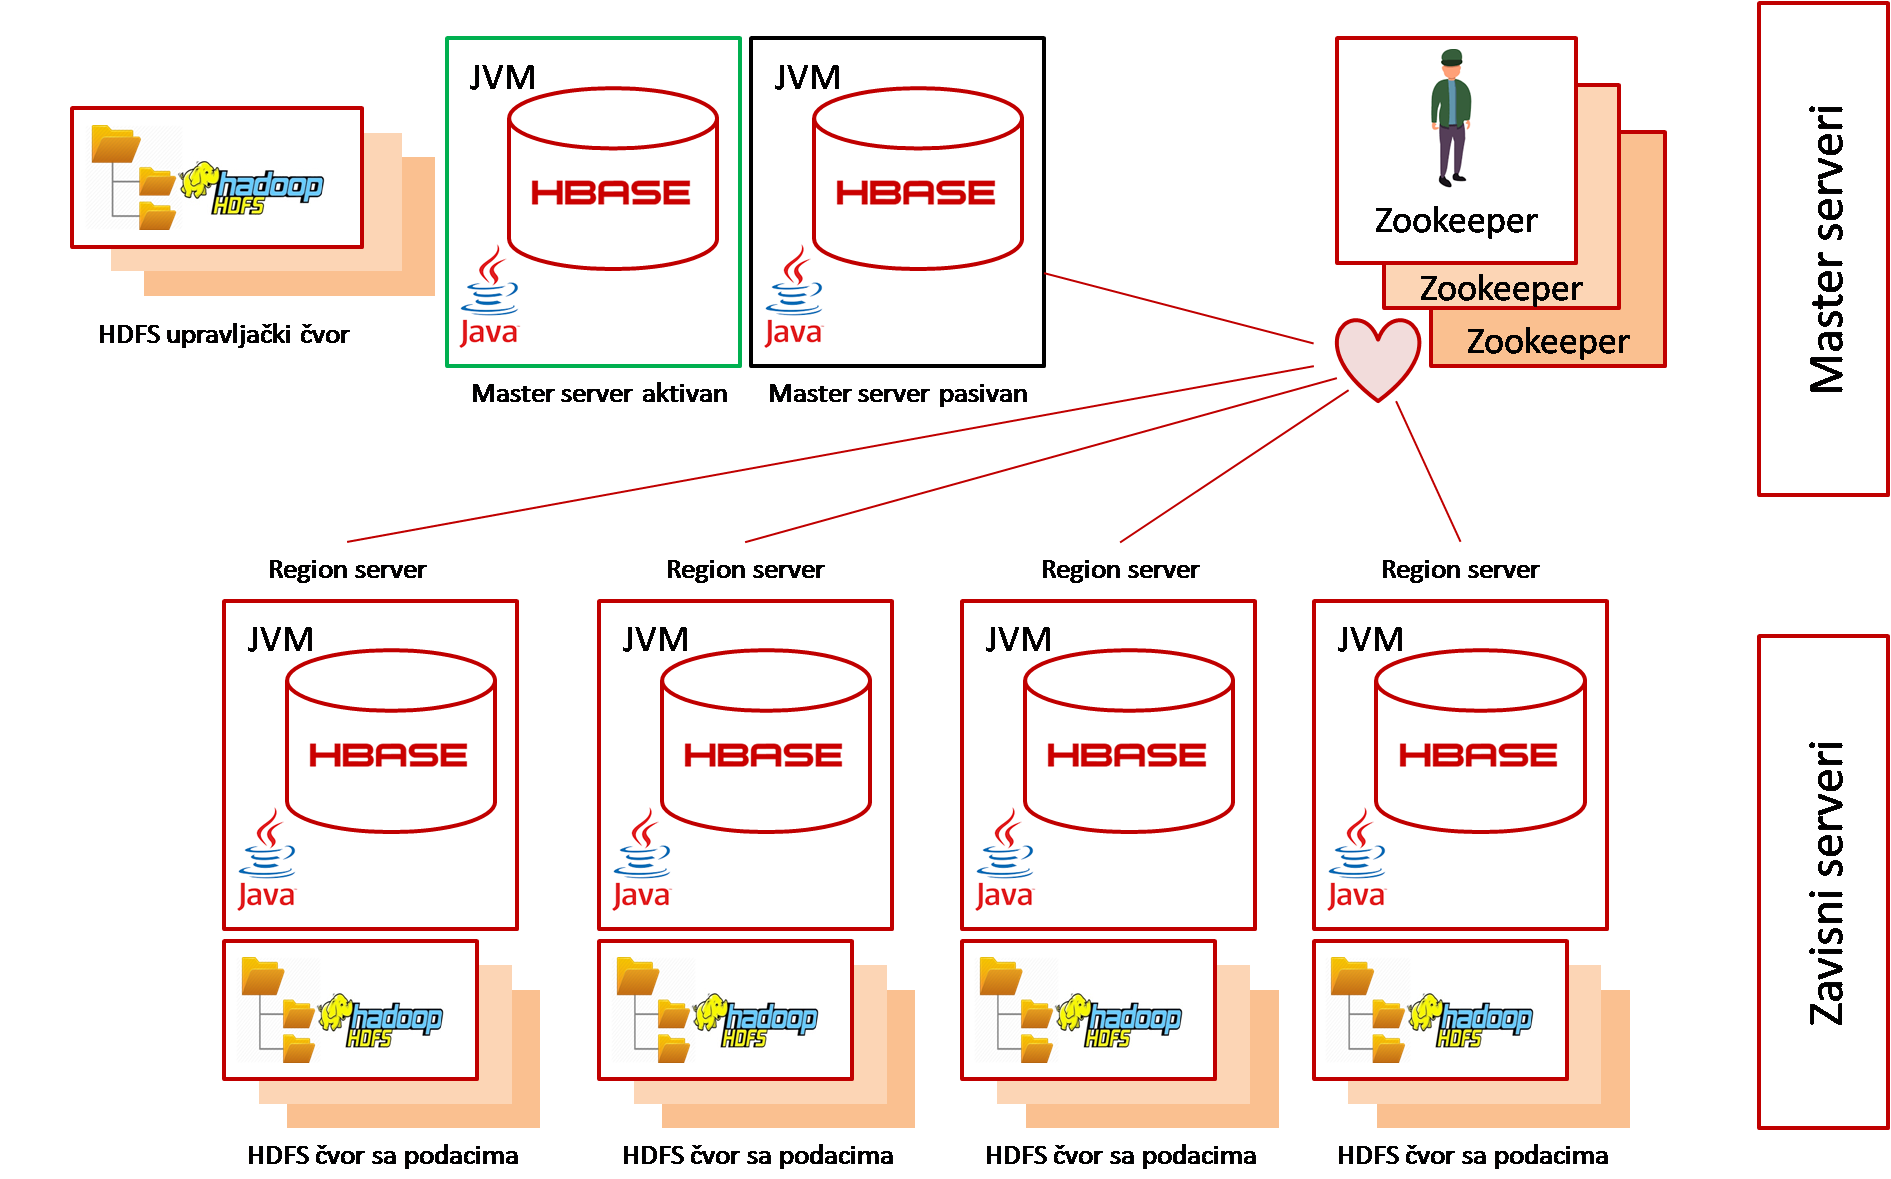
\includegraphics[width=0.9\textwidth]{hbase-distributed.png}
  \caption{HBase distributed}
  \label{fig:grafikon}
\end{figure}


\pagebreak

\section{Glavne razlike između relacionog i kolonski-orijentisanog modela}


\subsection{Normalizacija i denormalizacija}

U relacionim modelima često se radi na izbegavanju \textit{redudantnosti} u podacima. Redudantni podaci zauzimaju višak prostora na disku i otežavaju kasnije održavanje sistema. Kako bi se izbegla redudantnost postoje postupci koji nam pomažu da organizujemo podatke tako da redudantnost umanjimo. Proces izmene logičkog modela baze podataka u cilju rešavanja problea redundantosti podataka naziva se normalizacija. U zavisnosti od toga koja pravila zadovoljava određena relacija, dodeljuje joj se odgovarajuća normalna forma. Neke od normalnih formi relacionog modela su: 1. normalna forma, 2. normalna forma, 3. normalna froma, normalna forma elementarnog ključa, Bojs-Kodova normalna forma, 4. normalna forma, normalna forma esencijalnih torki, normalna forma bez redundansi, normalna forma superključeva, 5. normalna forma, normalna forma domena i ključa.

Normalizovani modeli obično raspolažu velikim brojem stranih ključeva što dovodi do povećanja broja tabela kojima se pristupa, a time i povećanja broja operacija čitanja sa diska što može uticati na performanse čitanja.

Denormalizacija je strategija koja se koristi kod modela kod kojih je neophodno ubrzati operacije čitanja podataka, odnosno umanjiti broj tabela kojima je neophodno pristupiti kako bi se neki skup podataka pročitao iz baze podataka.  

Neke od tehnika denormalizacije su:  spajanje kolone, horizontalna podela tabele, vertikalna podela tabele i uvođenje izvedene kolone. 

Spajanje kolone, slika 2.8. je dodavanje kolone kojoj bi se često pristupalo preko stranog ključa.

\begin{figure}[!ht]
  \centering
  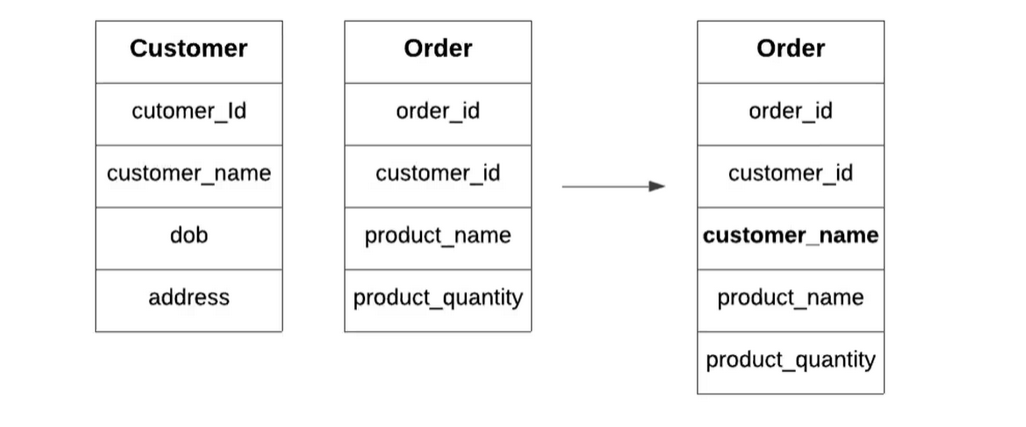
\includegraphics[width=0.9\textwidth]{denormalizacija.png}
  \caption{Spajanje kolone}
  \label{fig:grafikon}
\end{figure}

Horizontalno deljenje tabele, slika 2.9. podrazumeva da se na osnovu prirode podataka jedna tabela podeli na više tabela tako da se čitanje svede samo na čitanje grupe redova. 

\begin{figure}[!ht]
  \centering
  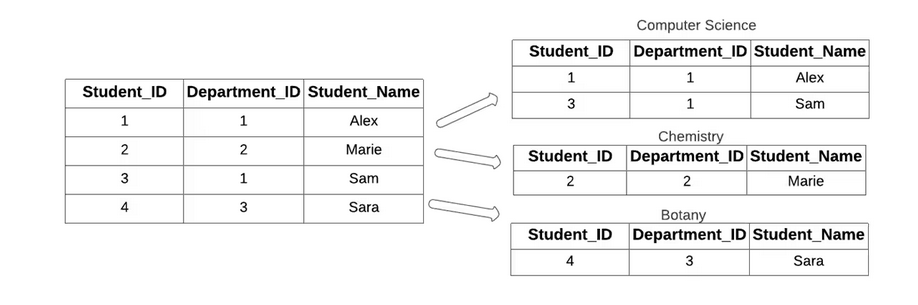
\includegraphics[width=0.9\textwidth]{denormalizacija2.png}
  \caption{Horizontalna podela tabele}
  \label{fig:grafikon}
\end{figure}

Vertikalno deljenje tabele, slika 2.10. podrazumeva da se tabela podeli grupisanjem kolona koje se često čitaju zajedno. 

\begin{figure}[!ht]
  \centering
  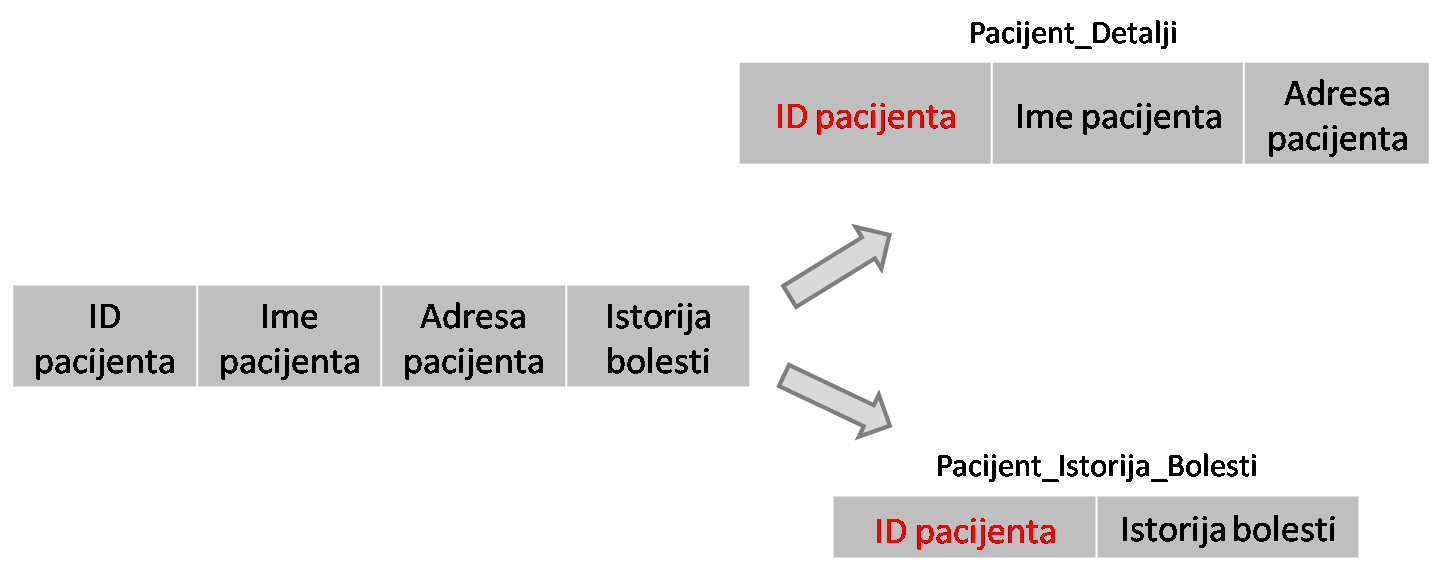
\includegraphics[width=0.9\textwidth]{denormalizacija3.png}
  \caption{Vertikalna podela tabele}
  \label{fig:grafikon}
\end{figure}

Uvođenje izvedene kolone, slika 2.11. predstavlja dodavanje kolone koja čuva rezultat neke agregatne funkcije. Time se izbegava da se pri svakom čitanju ta agregatna funkcija izvršava, već se pri ažuriranju stanja ta vrednost ažurira, da bi se rezultat kasnije mogao samo pročitati.



\begin{figure}[!ht]
  \centering
  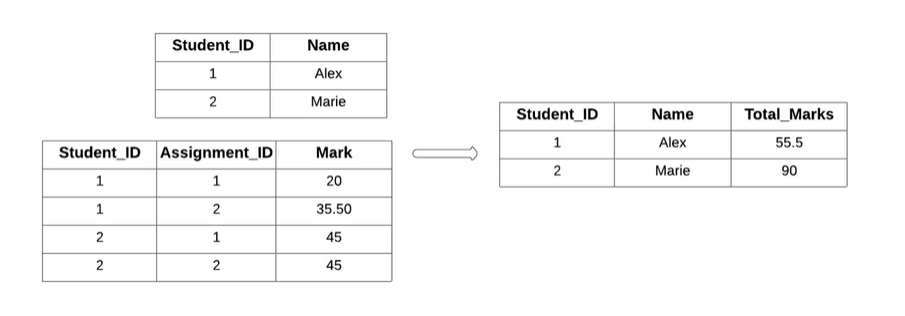
\includegraphics[width=0.9\textwidth]{denormalizacija4.png}
  \caption{Uvođenje izvedene kolone}
  \label{fig:grafikon}
\end{figure}
\pagebreak

\subsection{ACID i BASE}

Transakcija je logička jedinica posla pri radu sa podacima \cite{URBP}. Kod relacionih modela jednu transakciju karakteriše: atomičnost, konzistentost, izolovanost i trajnost (ACID).

Atomičnost transakcije se može objasniti pravilom: Jedna transakcija se izvršava u celini ili se ne izvršava nijedan njen deo, odnosno dejstvo transakcije je nedeljivo. 

Konzistentost transakcije znači da dejstvo transakcije ne može ostaviti stanje koje narušava integritet baze podataka.

Izolovanost transakcije čini da transakcije ne mogu uticati međusobno jedna na drugu, odnosno, kada se jedna transakcija pokrene, pa sve dok se ne završi, za nju, izmena neke druge transakcije neće biti vidljiva.

Trajnost transakcije garantuje da će kompletirana transakcija u slučaju prekida rada sistema pre nego što su izmene upisane na disk, biti upamćena i izvršena nakon restarta sistema. Svaka izmena se upisjue u log fajl pre nego što je upisana na disk, kako bi se operacije mogle poništiti u slučaju poništavanja transakcije.

Ova svojstva obično karakterišu transakcije u relacionom modelu, kada konzistentost baze ima nešto veći prioritet od brzine i dostupnosti. Kod kolonski orijentisanih baza podataka, posebno u distribuiranom režimu, dostupnost i brzina često imaju veći prioritet od stalne konzistentosti. Kod njih se koristi alternativni pristup karakterizacije transakcije - BASE. BASE transakcije zadovoljavaju sledeća svojstva: suštinska raspoloživost, postojanje mekog stanja i konvergentna konzistentnost.

Suštinska raspoloživost omogućava maksimalnu dostupnost čitanja i pisanja, ali bez garancije konzistentosti.

Meko stanje daje mogućnost da se stanje baze podataka menja čak i kada nijedna transakcija nije u toku, i to u periodu postizanja konzistetnosti.

Konvergentna konzistentnost obezbeđuje da će baza podataka u slučaju da nema novih upisa, postati konzistentna kroz neki vremenski period. 

\subsubsection{CAP teorema}

Kvalitet distribuiranih baza podataka ogleda se kroz tri svojstva: konzistentost, raspoloživost i tolerancija razdvojenosti.

Konzistenost u ovom kontekstu razlikuje se od konzistentosti transakcije. U kontekstu distribuiranih sistema, konzistetnost je svojstvo baze podataka, koje garantuje da će odgovor koji se šalje sa bilo kog čvora klastera (ukoliko odgovora ima) biti konzistentan .

Raspoloživost je svojstvo koje obezbeđuje da će baza uvek vratiti neki odgovor.

Tolerancija razdvojenosti znači da će u slučaju delimičniih otkaza unutar klastera, sistem i dalje vraćati ispravne odgovore.

CAP teorema koju je formulisao Eric Brewer  \footnote{Eric Allen Brewer profesor računarskih nauka na Univerzitetu Kalifornija, Berkli}, navodi da distribuirana baza podatka ne može istovremeno ispunjavati sva tri svojstva, slika 2.12.

Obzirom da je konzistentost i dostupnost u praksi skoro nemoguće dostići, distribuirane baze podataka organizuju se u skladu sa tim da li se veći prioritet daje dostupnosti ili stalnoj konzistentosti. Priroda sistema koji koriste relacioni model obično je takva da  daju prioritet konzistetnosti, pa se od relacionog modela očekuje da u distribuiranom okruženju osim konzistetnosti nudi i toleranciju razdvojenosti, za razliku od kolonski orijentisane nerelacione baze koja konzistetnost ne garantuje (garantuje konvergentnu konzistenciju), ali uz toleranciju razdvojenosti nudi stalnu dostupnost.

\begin{figure}[!ht]
  \centering
  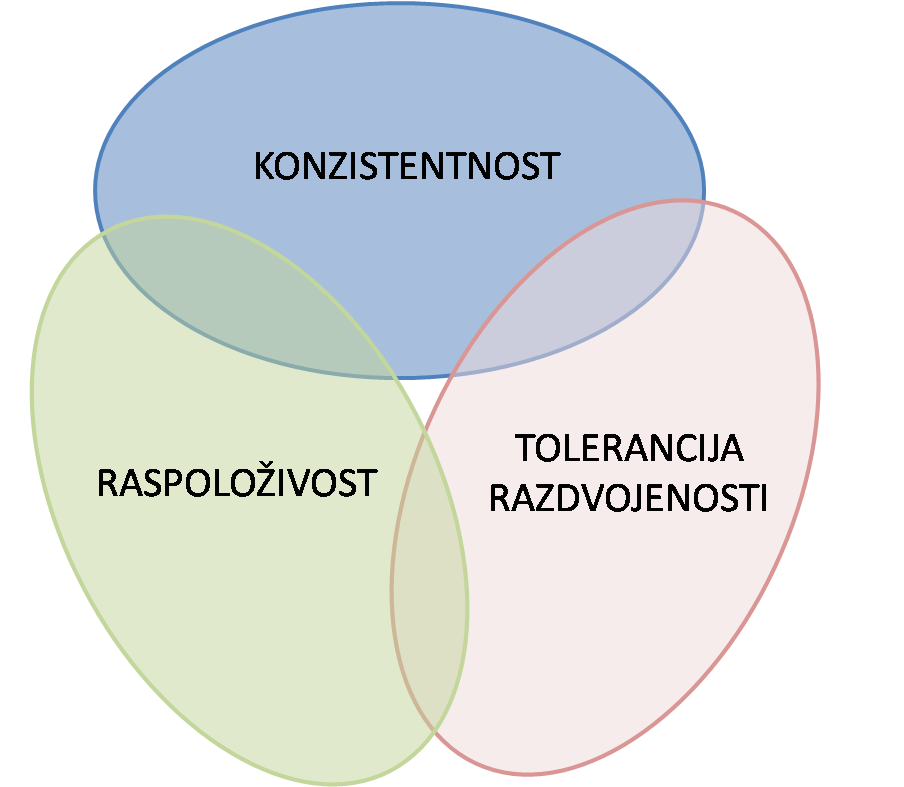
\includegraphics[width=0.9\textwidth]{cap.png}
  \caption{CAP teorema}
  \label{fig:grafikon}
\end{figure}

% ------------------------------------------------------------------------------
\chapter{Analiza slučajeva upotrebe}
% ------------------------------------------------------------------------------
\section{Opis i sadržaj eksperimenta}
Analiza i upoređivanje slučajeva upotrebe biće realizovani na osnovu teorijskih i praktičnih  izvora i istraživanja. Svaki primer će biti praćen eksperimentom koji će se sastojati od izvršavanja različitih vrsta postupaka.

U radu će biti analizirani sledeći slučajevi upotrebe:
\begin{enumerate}
\item Onlajn transakciono procesiranje (OLTP)
\item Onlajn analiticko procesiranje (OLAP)
\item Primena u distribuiranom okruženju
\end{enumerate}

Svakom slučaju upotrebe u okviru pripreme eksperimenata dodeljen je model podataka nad kojim se izvršavaju testovi.

Pored definisanja konteksta, analiza slučaja upotrebe sadržaće opis implementacije testova nad predstavnicima, uputstvo za pripremu okruženja kao i analizu rezultata.

Analiza rezultata eksperimenta će pored prikaza rezultata samih merenja, obuhvatiti i upoređivanje složenosti realizacije konkretnog slučaja upotrebe, kao i eventualna unapređenja i primedbe koje treba imati u vidu kada se radi sa datim tehnologijama. 

\subsection{Platforma testiranja}

Za predstavnike baza podataka čiji se modeli upoređuju i analiziraju izabrani su HBase i Postgres \footnote{Napomena: Kako su za predstavnike izabrani PostgresSQL i HBase, rezultati dobijeni u nastavku su rezultati poređenja konkretnih predstavnika, i nisu opšti za sve relacione i kolonski orijenisane nerelacione baze podataka.}.  Kao okruženje za izvršavanje eksperimenata korišćen je docker.Oba  predstavnika biće pokrenuta u okviru nezavisnih kontejnera na jednom računaru sa instaliranim docker-om. Svaki test predstavlja jedan java program koji se izvršava na konkretnom kontejneru, kako bi se smanjila potreba za evenutalnim saobraćajem kroz mrežu, a time i stekla što objektivnija slika na osnovu rezultata merenja. Dijagram sa opisom strukture platforme dat je na slici 3.1.




\begin{figure}[!ht]
  \centering
  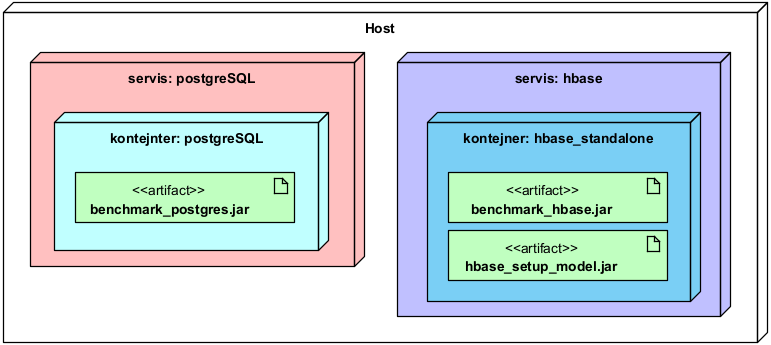
\includegraphics[width=0.9\textwidth]{deployment_diagram.png}
  \caption{Platforma testiranja}
  \label{fig:grafikon}
\end{figure}

\pagebreak

\section{Primena u online transakcionom procesiranju (OLTP)}

Onlajn transakciono procesiranje obuhvata kratke, učestale invazivne operacije na relativno malom skupu podataka. Da bismo simulirali ovakvo okruženje korišćen je primer onlajn transakcija i prenosa sredstava sa jednog računa na drugi. Parametri testa će biti broj biznis transakcija koje treba izvršiti, kao i broj klijenata, odnoso konekcija ka bazi, koji će paralelno obavljati svoj deo posla u okviru ovog testa. Jedna biznis transakcija sastoji se iz kreiranja transakcije, izvršavanja transakcije, odnosno prenos sredstava sa jednog računa na drugi, i na kraju provera statusa transakcije. 


\subsection{Opis modela}

Model koji ćemo koristiti sastojaće se iz 4 tabele:

\begin{enumerate}
\item[\textbullet] \textbf{fxrates}: {
	Sadrži informacije o kursu valutnih parova
}
\item[\textbullet] \textbf{fxuser}:{
	Podaci o korisnicima
}
\item[\textbullet] \textbf{fxaccount}:{
	Podaci o računima korisnika.
}
\item[\textbullet] \textbf{fxtransaction}:{
	Transakcije prenosa sredstava
}
\end{enumerate}

\lstset{
  language=sql,
  basicstyle=\footnotesize,
  keywordstyle=\color{black},
  backgroundcolor = \color{LemonChiffon1},
  numbers=left,
  showstringspaces=false,
  frame=single
}

\begin{lstlisting}[title={setup-postgres-model.sql},captionpos=t]

create table postgresdb.fxrates (
	currency_from  varchar(50) not null,
	currency_to varchar(50) not null,
	rate real not null,
	primary key(currency_from,currency_to)
);

create table postgresdb.fxuser (
	id  integer primary key,
	username varchar (50) unique not null,
	password varchar (50) not null,
	start_balancecurrency varchar (10) not null,
	start_balance real not null,
	firstname varchar(100) not null,
	lastname varchar(100) not null,
	street varchar(100) not null,
	city varchar(100) not null,
	state varchar(100) not null,
	zip varchar(50) not null,
	phone varchar(30) not null,
	mobile varchar(30) not null,
	email varchar(50) unique not null,
	created timestamp not null
);

create table postgresdb.fxaccount (
	id  integer primary key,
	fxuser integer not null  references postgresdb.fxuser(id),
	currency_code varchar(10) not null,
	balance real not null,
	created timestamp not null,
	unique (fxuser, currency_code)
);

create table postgresdb.fxtransaction (
	id integer primary key,
	fxaccount_from  integer references postgresdb.fxaccount(id),
	fxaccount_to  integer references postgresdb.fxaccount(id),
	amount numeric(15,2) not null,
	status varchar(50) not null,
	entry_date timestamp not null
);


\end{lstlisting}

\lstset{
  language=java,
  basicstyle=\footnotesize,
  keywordstyle=\color{black},
  backgroundcolor = \color{LemonChiffon1},
  numbers=left,
  showstringspaces=false,
  frame=single
}

\begin{lstlisting}[title={setup-hbase-model.sh},captionpos=t]
create fxrates, 'data';
create fxuser, 'data';
create fxaccount, 'data';
create fxtransaction, 'data';
\end{lstlisting}

\subsection{Implementacija testa}

Implementacija testa podrazumeva da ćemo imati dva parametra pri pokretanju: broj biznis transakcija koje će biti obrađene i broj klijenata koji će paralelno izvršavati svoj deo posla. Svakom klijentu će biti dodeljen određeni broj biznis transakcija koje treba da obradi. Svaka biznis transakcija sastoji se iz kreiranja transakcije (\textbf{createFXTransaction}), izvršavanja uplate (\textbf{executePayment}), provere statusa transakcije (\textbf{checkTransactionStatus}). 

CreateFXTransaction prvo pročita stanje naloga sa kojeg treba preneti sredstva, nakon toga čita odgovarajući kurs, a ukoliko ima dovoljno sredstava na računu u tabelu sa transakcijama upisuje transakciju u statusu NEW.

\lstset{
  language=sql,
  basicstyle=\footnotesize,
  keywordstyle=\color{black},
  backgroundcolor = \color{LemonChiffon1}
}

\begin{lstlisting}[title={CreateFXTransaction},captionpos=t]

select fa.balance
from fxaccount fa
where fa.id = ?;

select fr.rate
from fxrates fr
where fr.currency_to = ? and fr.currency_from = ?;

insert into fxtransaction
(id,fxaccount_from, fxaccount_to, amount, status, entry_date)
values(?,?,?,?,?,?)

\end{lstlisting}

ExecutePayment prvo pročita stanje sa naloga koji učestvuju u transakciji, menja im balans u skladu sa transakcijom, nakon toga transakciji menja status.



\lstset{
  language=sql,
  basicstyle=\footnotesize,
  keywordstyle=\color{black},
  backgroundcolor = \color{LemonChiffon1}
}

\begin{lstlisting}[title={ExecutePayment},captionpos=t]

select balance
from fxaccount
where id = ?

update fxaccount
set balance = ?
where id = ?

select balance
from fxaccount
where id = ?

update fxaccount
set balance = ?
where id = ?

update fxtransaction
set status = ?
where id = ?

\end{lstlisting}

CheckTransactionStatus za odgovarajucu transakciju čita status.

\lstset{
  language=sql,
  basicstyle=\footnotesize,
  keywordstyle=\color{black},
  backgroundcolor = \color{LemonChiffon1}
}

\begin{lstlisting}[title={CheckTransactionStatus},captionpos=t]
select status
from fxtransaction
where id = ?
\end{lstlisting}


Svaki klijent u zasebnoj niti obrađuje njemu dodeljen broj biznis transakcija, a svaka od njih se sastoji iz gore navedenih delova.

\lstset{
  language=Java,
  basicstyle=\footnotesize,
  keywordstyle=\color{black},
  backgroundcolor = \color{LemonChiffon1}
}

\begin{lstlisting}[title={BenchmarkSingleClientExecutor.java},captionpos=t]

public class BenchmarkSingleClientExecutor implements Runnable {

    private final CountDownLatch endSignal;
    private final BenchmarkOLTPUtility oltpUtil;
    private final int numOfT;
    private final int startFrom;

    private final Object connection;

    @Override
    public void run() {

       try {
         for (int i = this.start; i < this.start + this.numOfT; i++) {
             ExecutePaymentInfo executePaymentInfo = 
	    oltpUtil.createFXTransaction(connection);
	    oltpUtil.executePayment(,executePaymentInfo);
            oltpUtil.checkTransactionStatus(fxT);
          }
          endSignal.countDown();
        } catch (Exception e) {
            throw new IllegalStateException(e);
        }
    }
}

\end{lstlisting}



\subsection{Priprema okruženja}

S obzirom da se testovi izvršavaju na posebnim docker kontejnerima, potrebno  je da napravimo docker slike i pokrenemo kontejnere koristeći docker alat. Pored toga, neophodno je da kompajliramo java testove koristeći maven i nakon toga  prosledimo  odgovarajućim  kontejnerima.

\lstset{
  language=bash,
  basicstyle=\footnotesize,
  keywordstyle=\color{black},
  backgroundcolor = \color{LemonChiffon1}
}

\begin{lstlisting}[title={prepareEnv.sh},captionpos=t]
#!/bin/bash
echo 'PREPARING ENVIRONMENT...';

rm -f ./hbase_setup_model.jar
rm -f ./benchmark_hbase.jar
rm -f ./benchmark_postgres.jar

export JAVA_HOME="$JAVA_8";
mvn -f ./hbase_setup_model clean compile assembly:single;
mvn -f ./benchmark_hbase clean compile assembly:single;

export JAVA_HOME="$JAVA_17";
mvn -f ./benchmark_postgres clean compile assembly:single;


docker-compose -f docker-compose.yml up --build -d;
docker exec -it hbase-master-1 sh -c "java -jar hbase_setup_model.jar";

\end{lstlisting}

 Za pokretanje docker kontejnera korišćen je docker-compose sa sledećim sadržajem:

\lstset{
  basicstyle=\footnotesize,
  keywordstyle=\color{black},
  backgroundcolor = \color{LemonChiffon1},
  numbers=left,
  showstringspaces=false,
  frame=single
}

\begin{lstlisting}[title={docker-compose.yml},captionpos=t]
services: 
  postgres:
    container_name: postgres
    ports:
      - "5433:5432"
    volumes:
      - ./setup_model.sql:/docker-entrypoint-initdb.d/create_script.sql
      - ./benchmark_postgres.jar:/benchmark_postgres.jar
    environment:
      - POSTGRES_PASSWORD=postgres
      - POSTGRES_USER=postgres
      - POSTGRES_DB=postgresdb
    build:
      context: .
      dockerfile: ./Dockerfile_postgres

  hbase:
    image: bde2020/hbase-standalone:1.0.0-hbase1.2.6
    container_name: hbase
    volumes:
      - hbase_data:/hbase-data
      - hbase_zookeeper_data:/zookeeper-data
      - ./hbase_setup_model.jar:/hbase_setup_model.jar
      - ./benchmark_hbase.jar:/benchmark_hbase.jar
    ports:
      - 16000:16000
      - 16010:16010
      - 16020:16020
      - 16030:16030
      - 2888:2888
      - 3888:3888
      - 2181:2181

volumes:
  hbase_data:
  hbase_zookeeper_data:
\end{lstlisting}


\subsection{Analiza rezultata}

Kada se radi o OLTP okruženju, važno je naglasiti da HBase ne garantuje konzistentost nad svim podacima kakvu nudi Postgres. HBase ipak garantuje neki vid konzistentosti, tj konzistentost nad jednim redom tabele. To dovodi do zaključka da ukoliko je neophodno implementirati transakciju koja uključuje rad sa podacima više tabela ili više redova jedne tabele, ukoliko koristimo HBase moramo na aplikativnom sloju voditi računa o očuvanju  eventualne konzistetnosti. Postgres sa druge strane kao ACID baza sama garantuje da izmene neke transakcije koje se rade nad nekim skupom podataka neće biti vidljive za druge klijente dok se ta transakcija ne komituje, pa samim tim i konzistento stanje podataka.

\begin{figure}[!ht]
  \centering
  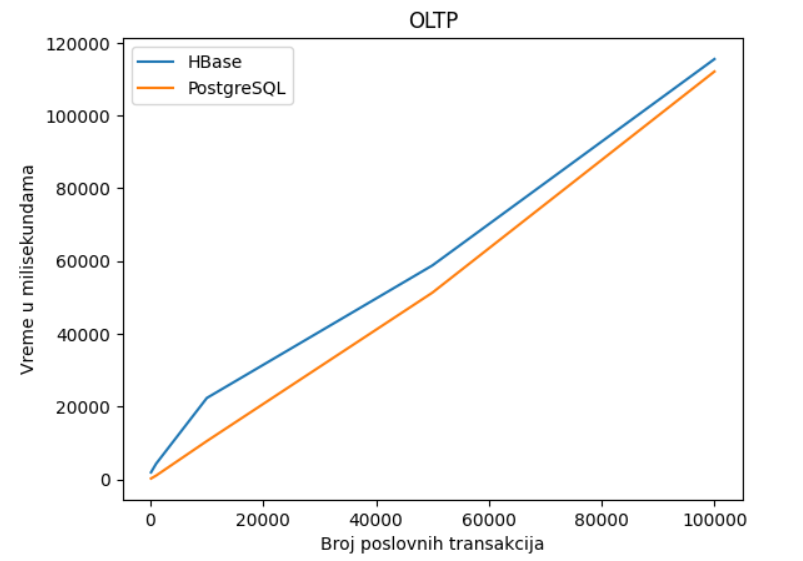
\includegraphics[width=0.8\textwidth]{oltp-vizualization.png}
  \caption{Rezultati merenja u OLTP okruženju}
  \label{fig:grafikon}
\end{figure}

\begin{figure}[!ht]
  \centering
  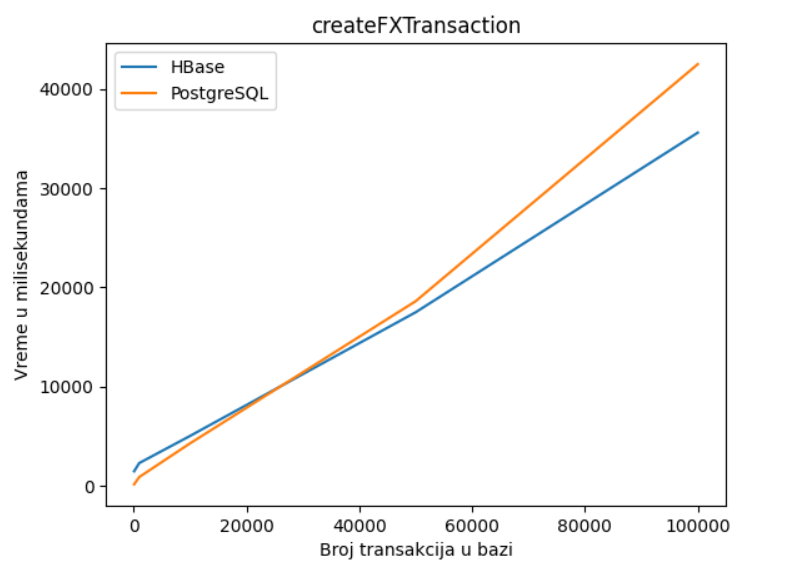
\includegraphics[width=0.8\textwidth]{createFxTransaction-vizualization.png}
  \caption{Rezultati merenja createFXTransaction dela biznis transakcije}
  \label{fig:grafikon}
\end{figure}

Merenje efikasnosti predstavnika u OLTP okruženju uključivalo je pokretanje testova u više iteracija. Svaki test je podrazumevao 5 klijenata koji paralelno obaljaju svoj deo posla, a pokrenuti su testovi za obradu \numprint{100},\numprint{1000}, \numprint{10000},\numprint{50000},\numprint{100000} biznis transakcija, a rezultati merenja prikazani su na slici 3.2. Primećuje se da sa porastom podataka koji se nalaze u tabeli sa čijim se podacima radi, Postgres ima određena usporenja, relativno gledano u odnosu na HBase. Konkretno kada se pogleda vreme delova biznis transakcije odvojeno, primećuje se da HBase u testovima sa \numprint{50000} i \numprint{100000} iteracija prednost stiče u createFXTransaction delu cele biznis transakcije, što se može videti na slici 3.3. 

Tendencija merenja ukazuje da bi sa porastom broja podataka (na milione i desetine miliona redova) HBase davao bolje rezultate u odnosu na Postgres, međutim za testiranje takvog okruženja neophodno je koristiti računar koji je sposoban da sprovede tako zahtevan test.


\section{Primena u online analitičkom procesiranju (OLAP)}

OLAP okruženje sačinjeno je od velikog broja čitanja podataka i vrlo malog broja izmena podataka.. Upiti koji se koriste obično imaju parametre, visok nivo kompleksnosti i visok procenat podataka kojima pristupaju.
Primer koji emo koristiti jeste uopšten primer održavanja trgovinskog lanca koji ima skup mušterija, proizvoda, dobavljača,  narudžbina. 
Ovaj OLAP eksperiment će se sastojati iz dohvatanja izveštaja iz tabele koja sadrži stavke narudžbina. Taj izveštaj će sadržati rezultate agregiranih operacija nad kolonama, a parametri će biti status i datum slanja stavke.

\subsection{Modeli podataka}

Model koji ćemo koristiti sastojaće se iz sledećih tabela:

\begin{enumerate}
\item[\textbullet] \textbf{product}: {
	Sadrži informacije o proizvodima. Predviđeno je da sadrži 3000000 redova.
}
\item[\textbullet] \textbf{supplier}:{
	Podaci o dovaljačima. Predviđeno je da sadrži 1000000 redova.
}
\item[\textbullet] \textbf{productsupplier}:{
	Vezna tabela između dobavljača i proizvoda. Predviđeno je da sadrži 5000000 redova.
}
\item[\textbullet] \textbf{customer}:{
	Informacije o mušterijama. Predviđeno je da sadrži 1500000 redova.
}
\item[\textbullet] \textbf{order}:{
	Informacije o narudžbinama. Predviđeno je da sadrži 1500000 redova.
}
\item[\textbullet] \textbf{orderitem}:{
	Informacije o pojedinim stavkama narudžbine. Predviđeno je da sadrži 6000000 redova.
}

\end{enumerate}


\lstset{
  language=sql,
  basicstyle=\footnotesize,
  keywordstyle=\color{black},
  backgroundcolor = \color{LemonChiffon1},
  numbers=left,
  showstringspaces=false,
  frame=single
}

\begin{lstlisting}[title={setup-postgres-model.sql},captionpos=t]


create table product (
    id  integer not null primary key,
    name varchar(50) not null,
    brand varchar(50) not null,
    type varchar(50) not null,
    size integer not null,
    container varchar(50) not null,
    price varchar(50) not null,
    comment varchar(50)
);

create table supplier (
    id  integer primary key,
    name varchar(50) not null,
    address varchar(200) not null,
    phone varchar(50) not null
);

create table productsupplier (
    id integer not null primary key,
    product integer not null,
    supplier integer not null,
    available integer not null,
    supply_cost real not null,
    comment varchar(200),
    constraint fk_product
    foreign key(product) references  postgresdb.product(id),
    constraint fk_supplier
    foreign key(supplier) references  postgresdb.supplier(id)
    
);

create table customer(
    id integer primary key,
    name varchar(50) not null,
    address varchar(200) not null,
    phone varchar(50) not null,
    comment varchar(200)
);

create table order(
    id integer primary key,
    customer integer not null,
    status varchar(20) not null,
    total_price real not null,
    entry_date date not null,
    priority varchar(20) not null,
    comment varchar(200),
    constraint fk_customer
    foreign key(customer) references  postgresdb.customer(id)
);

create table order_item(
    order_id integer not null,
    product integer not null,
    supplier integer not null, 
    order_no integer not null,
    quantity integer not null,
    base_price real not null,
    discount real not null,
    tax real not null,
    status varchar(20) not null,
    ship_date date not null,
    commit_date date not null,
    comment varchar(200),
    primary key(order_id,product,supplier),
    constraint fk_order
    foreign key(order_id) references  postgresdb.order(id),
    constraint fk_product
    foreign key(product) references  postgresdb.product(id),
    constraint fk_supplier
    foreign key(supplier) references  postgresdb.supplier(id)
);

\end{lstlisting}


\lstset{
  language=java,
  basicstyle=\footnotesize,
  keywordstyle=\color{black},
  backgroundcolor = \color{LemonChiffon1},
  numbers=left,
  showstringspaces=false,
  frame=single
}

\begin{lstlisting}[title={hbase-setup-model},captionpos=t]

create product, 'data';
create supplier, 'data';
create productsupplier, 'data';
create customer, 'data';
create order, 'data';
create orderitem, 'data';

\end{lstlisting}

\subsection{Implementacija testa}

Test će se sastojati iz dve faze. Bulk upunjavanje tabela na osnovu csv fajlova, kao i izvršavanje složenog OLAP upita. 

\lstset{
  language=sql,
  basicstyle=\footnotesize,
  keywordstyle=\color{black},
  backgroundcolor = \color{LemonChiffon1},
  numbers=left,
  showstringspaces=false,
  frame=single
}
\begin{lstlisting}[title={bulkLoad},captionpos=t]
copy product from "./product.csv";
copy supplier from "./supplier.csv";
copy productsupplier "./productsupplier.csv";
copy customer from "./customer.csv";
copy order from "./order.csv";
copy order_item from "./order_item.csv";
\end{lstlisting}

\lstset{
  language=java,
  basicstyle=\footnotesize,
  keywordstyle=\color{black},
  backgroundcolor = \color{LemonChiffon1},
  numbers=left,
  showstringspaces=false,
  frame=single
}

\begin{lstlisting}[title={BenchmarkExecutor.java},captionpos=t]

    void bulkLoad(BenchmarkUtility util,BenchmarkOLAPUtility oUtil) {
        long start = System.currentTimeMillis();
        olapUtility.bulkLoad(benchmarkUtility.connect());
        long end = System.currentTimeMillis();
        System.out.println("Bulk load duration: "+(end-start));
    }
\end{lstlisting}


OLAP upit sadrži informacije o agregiranim vrednostima kolona za određene vrednosti kolona. Upit će se izvršavati nad orderitem tabelom, a kao parametre uzimaće status i datum slanja stavke narudžbine.

\lstset{
  language=java,
  basicstyle=\footnotesize,
  keywordstyle=\color{black},
  backgroundcolor = \color{LemonChiffon1},
  numbers=left,
  showstringspaces=false,
  frame=single
}

\begin{lstlisting}[title={executeOLAPQuery},captionpos=t]

select
	oi.status status,
	sum(oi.quantity) as sum_qty,
        sum(oi.base_price) as sum_base_price,
        sum(oi.base_price*(1-oi.discount)) as sum_disc_price,
        sum(oi.base_price*(1-oi.discount)*(1+oi.tax)) as sum_charge,
        avg(oi.quantity) as avg_qty,
        avg(oi.base_price) as avg_price,
        avg(oi.discount) as avg_disc,
        count(*) as count_order
from
         postgresdb.order_item oi
where
        	oi.ship_date = to_date(?,'dd.mm.yyyy') and
         oi.status = ?

\end{lstlisting}

Parametri eksperimenta će biti broj iteracija izvršavanja OLAP upita kao i broj klijenata koji će paralelno izvršavati svoj deo posla u vidu određenog broja izvršavanja OLAP upita.


\lstset{
  language=java,
  basicstyle=\footnotesize,
  keywordstyle=\color{black},
  backgroundcolor = \color{LemonChiffon1},
  numbers=left,
  showstringspaces=false,
  frame=single
}

\begin{lstlisting}[title={BenchmarkSingleClientExecutor.java},captionpos=t]

public class BenchmarkSingleClientExecutor implements Runnable{

    private final CountDownLatch endSignal;
    private final BenchmarkOLAPUtility olapUtil;
    private final int numOfT;
    private final int start;

    private final Object connection;

    @Override
    public void run() {
        try {
            for (int i = this.start; i < this.start+this.numOfT; i++) {
                olapUtil.executeOLAPQuery(connection);
            }
            endSignal.countDown();
        } catch (Throwable e) {
            throw new IllegalStateException(e);
        }
    }
}

\end{lstlisting}

\subsection{Priprema okruženja}

Priprema okruženja je većinom identična kao priprema okruženja za OLTP slučaj upotrebe. Dodatan korak jedino je kreiranje csv fajlova sa podacima koji treba da budu bulk učitani u odgovarajuće tabele Postgres-a i HBase-a.
\pagebreak
\lstset{
  language=java,
  basicstyle=\footnotesize,
  keywordstyle=\color{black},
  backgroundcolor = \color{LemonChiffon1},
  numbers=left,
  showstringspaces=false,
  frame=single
}

\begin{lstlisting}[title={prepareEnv.sh},captionpos=t]
#!/bin/bash
echo 'PREPARING ENVIRONMENT...';
rm -f ./olap_benchmark_postgres.jar
rm -f ./olap_benchmark_hbase.jar
rm -f ./productHB.csv;
rm -f ./supplierHB.csv;
rm -f ./productsupplierHB.csv;
rm -f ./customerHB.csv;
rm -f ./orderHB.csv;
rm -f ./orderitemHB.csv;
rm -f ./productPG.csv;
rm -f ./supplierPG.csv;
rm -f ./productsupplierPG.csv;
rm -f ./customerPG.csv;
rm -f ./orderPG.csv;
rm -f ./orderitemPG.csv;


echo 'PREPARING HBASE BENCHMARK JARS...';
export JAVA_HOME="$JAVA_8";
mvn -f olap_benchmark_hbase clean compile assembly:single;
mvn -f hbase_setup_olap_model clean compile assembly:single;
mvn -f hbase_bulk_load_setup clean compile assembly:single;

echo 'PREPARING HBASE BULK LOAD RESOURCES..';
java -jar ./hbase_bulk_load_setup.jar;


echo 'PREPARING POSTGRES BENCHMARK JARS...';
export JAVA_HOME="$JAVA_17";
mvn -f olap_benchmark_postgres clean compile assembly:single;
mvn -f postgres_bulk_load_setup clean compile assembly:single;

echo 'PREPARING POSTGRES BULK LOAD RESOURCES..';
java -jar postgres_bulk_load_setup.jar;

docker-compose -f docker-compose.yml up --build -d;
winpty docker exec -it hbase sh -c "java -jar setup_olap_model.jar";

\end{lstlisting}


\pagebreak

 Za pokretanje docker kontejnera korišćen je docker-compose sa sledećim sadržajem:

\lstset{
  language=java,
  basicstyle=\footnotesize,
  keywordstyle=\color{black},
  backgroundcolor = \color{LemonChiffon1},
  numbers=left,
  showstringspaces=false,
  frame=single
}

\begin{lstlisting}[title={docker-compose.yml},captionpos=t]

services: 
  postgres:
    container_name: postgres
    ports:
      - "5433:5432"
    volumes:
      - ./setup_model.sql:/docker-entrypoint-initdb.d/create_script.sql
      - ./benchmark_postgres.jar:/benchmark_postgres.jar
    environment:
      - POSTGRES_PASSWORD=postgres
      - POSTGRES_USER=postgres
      - POSTGRES_DB=postgresdb
    build:
      context: .
      dockerfile: ./Dockerfile_postgres

  hbase:
    image: bde2020/hbase-standalone:1.0.0-hbase1.2.6
    container_name: hbase
    volumes:
      - ./productsupplierHB.csv:/productsupplier.csv
      - ./productHB.csv:/product.csv
      - ./supplierHB.csv:/supplier.csv
      - ./customerHB.csv:/customer.csv
      - ./orderHB.csv:/order.csv
      - ./orderitemHB.csv:/orderitem.csv
      - ./orderitemStatsHB.csv:/orderitemstats.csv
      - hbase_data:/hbase-data
      - hbase_zookeeper_data:/zookeeper-data
      - ./hbase_setup_model.jar:/hbase_setup_model.jar
      - ./benchmark_hbase.jar:/benchmark_hbase.jar
    ports:
      - 16000:16000
      - 16010:16010
      - 16020:16020
      - 16030:16030
      - 2888:2888
      - 3888:3888
      - 2181:2181

volumes:
  hbase_data:
  hbase_zookeeper_data:
\end{lstlisting}


\subsection{Analiza rezultata}

Rezultati merenja u OLAP okruženju ,kada se koriste ravnopravni modeli pokazuju jasnu prednost Postgres-a u odnosu na HBase. Sa druge strane, ovakav pristup gde se čitaju svi redovi filtrirani po statusu i datumu, pa se nad vrednostima izvršavaju odgovarajuće aritmetičke operacije, može se nazvati \textit{"naivnim"} u slučaju HBase-a. 

Jednostavna denormalizacija modela, slika 3.4 može doneti dramatična poboljšanja u performansama HBase-a čak i u odnosu na Postgres.

\begin{figure}[!ht]
  \centering
  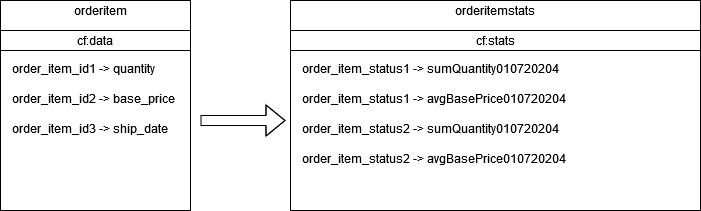
\includegraphics[width=1\textwidth]{denormalized-model.png}
  \caption{Denormalizacija na primeru tabele orderitem}
  \label{fig:grafikon}
\end{figure}

Izdvajanje tabele \textbf{orderitemstats}, koja će za ključ imati status stavke, a kao kolone imati rezultate već ranije izračunatih agregatnih vrednosti nad kolonama za odgovarajuče dane, dovodi do toga da čitanje izveštaja sada predstavlja jednostavno čitanje reda po ključu i skupa odgovarajućih kolona koje su nam potrebne za izveštaj.

Uticaj denormalizacije modela na performanse mogu se videti na slici 3.5.

\begin{figure}[!ht]
  \centering
  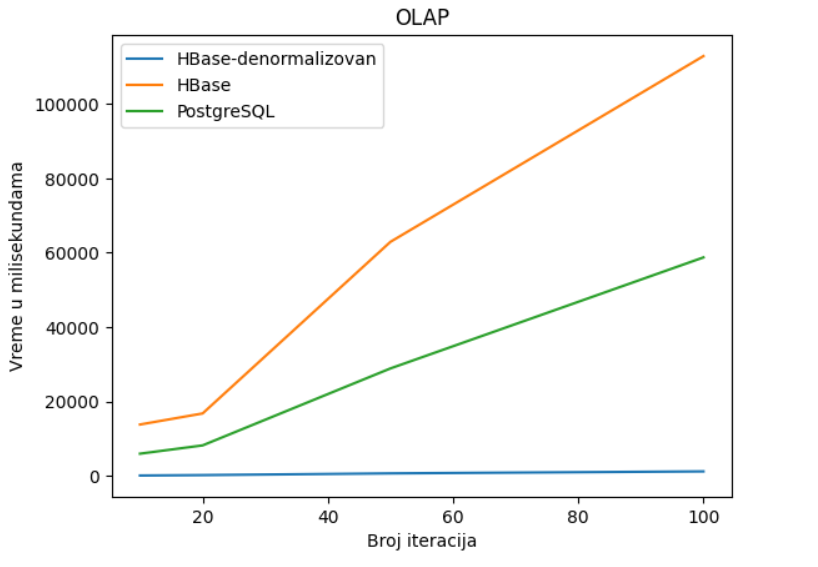
\includegraphics[width=1\textwidth]{olap-vizualization.png}
  \caption{Uporedna analiza performansi postgresa i hbase-a}
  \label{fig:grafikon}
\end{figure}

Ovakav pristup prilikom kreiranja modela, omogućila nam je fleksibilnost strukture koju HBase nudi, kao i nepostojanje limita broja kolona. 

\pagebreak


\section{Primena u distribuiranom okruženju}


Distribuirano okruženje odlikuje 

\chapter{Zaključak}

% ------------------------------------------------------------------------------
% Literatura
% ------------------------------------------------------------------------------
\literatura

% ==============================================================================
% Završni deo teze i prilozi
\backmatter
% ==============================================================================

% ------------------------------------------------------------------------------
% Biografija kandidata
\begin{biografija}
\textbf{Вук Стефановић Караџић} (\emph{Тршић, 26. октобар/6. новембар
  1787. — Беч, 7. фебруар 1864.}) био је српски филолог, реформатор
српског језика, сакупљач народних умотворина и писац првог речника
српског језика.  Вук је најзначајнија личност српске књижевности прве
половине XIX века. Стекао је и неколико почасних доктората.
Учествовао је у Првом српском устанку као писар и чиновник у
Неготинској крајини, а након слома устанка преселио се у Беч,
1813. године. Ту је упознао Јернеја Копитара, цензора словенских
књига, на чији је подстицај кренуо у прикупљање српских народних
песама, реформу ћирилице и борбу за увођење народног језика у српску
књижевност. Вуковим реформама у српски језик је уведен фонетски
правопис, а српски језик је потиснуо славеносрпски језик који је у то
време био језик образованих људи. Тако се као најважније године Вукове
реформе истичу 1818., 1836., 1839., 1847. и 1852.
\end{biografija}
% ------------------------------------------------------------------------------

\end{document} 